\begin{surferPage}[Cúspide A2++]{Una altra cúspide (singularitat $A_2^{++}$)}
És similar a la cúspide anterior.
La seva equació és la mateixa, llevat d'un canvi de signe:
    \vspace*{-0.4em}
    \begin{center}
      $x^3+y^2+z^2=0.$
    \end{center}
    \vspace*{-0.4em}
Aquest canvi dóna una superfície de revolució (no canvia per
girs al voltant de l'eix $x$), com també ho és la seva deformació
    $(1-a)x^3-ax^2+y^2+z^2=0$, $a>0$
en una singularitat del tipus $A_1^{+-}$:
    \begin{center}
      \vspace*{-0.6em}
      \begin{tabular}{@{}c@{\quad}c@{\quad}c@{}}
        \begin{tabular}{@{}c@{}}
          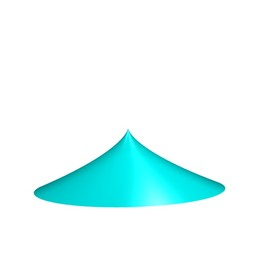
\includegraphics[width=1.2cm]{../../common/images/A2pp_0}
        \end{tabular}
        &
        \begin{tabular}{@{}c@{}}
          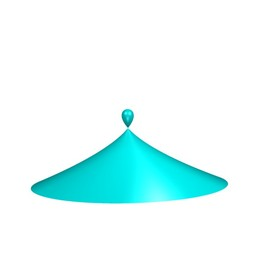
\includegraphics[width=1.2cm]{../../common/images/A2pp_1}
        \end{tabular}
        &
        \begin{tabular}{@{}c@{}}
          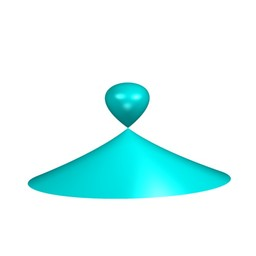
\includegraphics[width=1.2cm]{../../common/images/A2pp_2}
        \end{tabular}
      \end{tabular}
    \end{center}
    \vspace*{-0.5em}
Remarquem que si escrivim l'equació en la forma
$y^2+z^2=-(x^3)$, que mostra que per a un valor fixat
$x<0$ s'obté una circumferència ($y^2+z^2=r^2$ representa una
circumferència de radi $r$, pel teorema de Pitàgores).
El tall de la cúspide deformada pel pla $z=0$ dóna una cúspide plana
(si $a=0$) o un llaç (si $a\neq0$).
    \begin{center}
      \vspace*{-0.7em}
      \begin{tabular}{@{}c@{\quad}c@{\quad}c@{}}
        \begin{tabular}{@{}c@{}}
          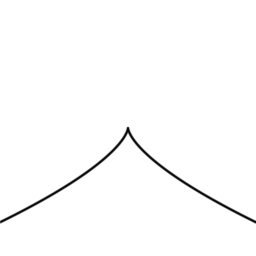
\includegraphics[width=1.2cm]{../../common/images/cuspe_def_cut_1}
        \end{tabular}
        &
        \begin{tabular}{@{}c@{}}
          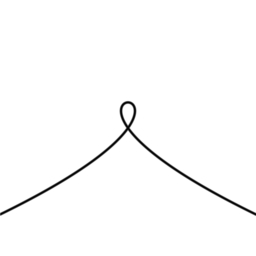
\includegraphics[width=1.2cm]{../../common/images/cuspe_def_cut_2}
        \end{tabular}
        &
        \begin{tabular}{@{}c@{}}
          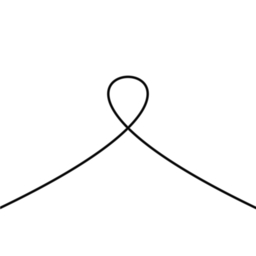
\includegraphics[width=1.2cm]{../../common/images/cuspe_def_cut_3}
        \end{tabular}
      \end{tabular}
    \end{center}
 
\end{surferPage}
